%======================================================================
\section{Cuánto riesgo queda: el estimador de Rao--Blackwell}\label{sec:riesgo-rb}
%======================================================================
\paragraph{El problema.} Ninguna variante de N2 cruzó 1220~K en las 60 realizaciones de la
sección~\ref{sec:riesgo-cota}. Contar cruces sólo acotaba la probabilidad bajo el 6\,\% y no
permitía comparar variantes. Para comparar probabilidades del orden de 1\,\% con un error
relativo del 10\,\% contando cruces harían falta del orden de $10^4$ realizaciones.

\paragraph{La idea: integrar en vez de sortear.} En una corrida sin fallas de cada
controlador se conoce su trayectoria $x_t$. Si la \emph{primera} falla del sistema empieza en
$t$ (densidad $\lambda e^{-\lambda t}$, proceso de Poisson) y dura $D$, hay cruce si y sólo si
$D>\tau(x_t)$, donde $\tau(x_t)$ es lo que tarda \textbf{el HRM} (la planta, no el ROM) en pasar
1220~K con el ACS apagado desde $x_t$ (\code{time\_to\_limit}). La duración no hace falta
sortearla, porque su distribución se conoce:
\[
P(\text{cruce})=\int_0^T\lambda e^{-\lambda t}\,S\big(\tau(x_t)\big)\,dt,\qquad
S(\tau)=\sum_i w_ie^{-\mu_i\tau}.
\]
Es un estimador de \emph{Rao--Blackwell}: reemplaza la variable indicadora del cruce por su
esperanza condicional dada la trayectoria. Por el teorema de Rao--Blackwell, condicionar no
cambia la media y no aumenta la varianza~\cite{casella2002}; aquí la reduce mucho, porque toda la
aleatoriedad de $D$ se integra en forma exacta. Es exacto para la primera falla e ignora las
siguientes, que son de segundo orden. La versión condicionada a una falla en $[0,220]$~s divide
por $1-e^{-220\lambda}$. Implementación: \code{julia/f5b1c\_rb\_risk.jl}, con $\tau$ evaluado
cada 5~s (cada 10~s en la campaña F6).

\paragraph{Validación.} Para el PI del DET, el estimador da $0.119\pm0.016$, y el conteo directo
de la sección~\ref{sec:riesgo-cota} había dado 7/60 = 0.117. Para N2 da $0.031\pm0.004$,
compatible con 0/60.

\begin{table}[H]\centering\footnotesize\setlength{\tabcolsep}{4pt}
\begin{tabularx}{\linewidth}{@{}Y r r r r@{}}\toprule
Caso (50 realizaciones) & $P(\text{cruce}\mid\text{falla})$ & Cociente vs N2 (IC 95\,\%) & K bajo $y_{\rm ref}$ & Masa\\\midrule
N2+sesgo & $0.031\pm0.004$ & 1 & $-0.1$ & ---\\
N2+cota, $\alpha=0.05$ & $0.027\pm0.002$ & 0.91 [0.87, 0.95] & 1.1 & +2\,\%\\
N2+cota, $\alpha=0.02$ & $0.015\pm0.001$ & 0.53 [0.50, 0.57] & 7.5 & +17\,\%\\
N2+cota, $\alpha=0.01$ & $0.011\pm0.001$ & 0.37 [0.35, 0.39] & 12.9 & +32\,\%\\
PID de la tesis & $0.033\pm0.004$ & 1.05 [1.03, 1.06] & 0.1 & +1\,\%\\
PI del DET & $0.119\pm0.016$ & 3.78 [3.76, 3.80] & $-6.8$ & +48\,\%\\\bottomrule
\end{tabularx}
\caption{Probabilidad de llegar a 1220~K dada una falla del ACS (40~kg/s, fallas del DET con
$\mu\times10^4$), estimada por Rao--Blackwell sobre trayectorias sin fallas (semillas 201--250).
«K bajo $y_{\rm ref}$»: desvío medio de la PCT bajo la consigna, el costo de pre-enfriar. La
campaña F6 repitió estos casos con las mismas semillas y obtuvo los mismos valores (0.0312,
0.0270, 0.0155, 0.0110, 0.0326 y 0.1185).}
\label{tab:rb}
\end{table}

\begin{figure}[H]\centering
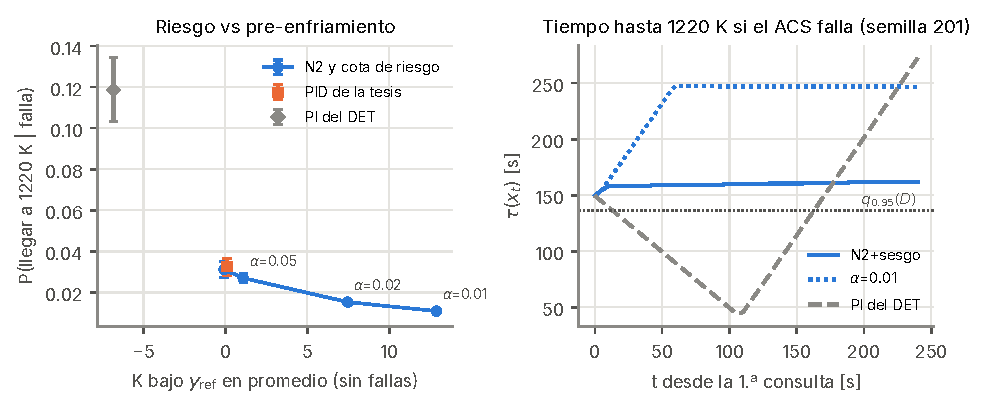
\includegraphics[width=\linewidth]{figures/fig_f5b_rb_risk.pdf}
\caption{Izquierda: frontera riesgo--pre-enfriamiento. Derecha: con $\alpha=0.01$, N2 mantiene el
tiempo hasta 1220~K sobre $q_{0.99}(D)\approx219$~s; sin cota queda en $\approx160$~s, y el PI del
DET baja hasta 45~s.}
\end{figure}

\paragraph{Cómo leer la tabla.}
\begin{enumerate}
  \item \textbf{La cota cumple su garantía nominal.} $P(\text{cruce}\mid\text{falla})$ queda bajo
        $\alpha$: 0.027 con $\alpha=0.05$, 0.015 con $\alpha=0.02$ y 0.011 con $\alpha=0.01$, este
        último en el límite. Con $\alpha=0.10$ la cota no hace nada, porque N2 ya está en 0.031.
  \item \textbf{Hay un piso de 0.002.} El 0.2\,\% de las fallas (la componente de 2.9~h) dura
        más que cualquier transitorio, y ningún controlador lo evita.
  \item \textbf{El precio es pre-enfriar.} Bajar el riesgo a la mitad ($\alpha=0.02$) cuesta
        trabajar 7.5~K bajo la consigna y un 17\,\% más de masa; bajarlo a un tercio
        ($\alpha=0.01$), 12.9~K y 32\,\%.
  \item \textbf{Contra el mismo criterio,} el PID de la tesis es un 5\,\% más riesgoso que N2 y
        el PI del DET casi 4 veces más.
  \item \textbf{Por transitorio} de 240~s con las tasas aceleradas, N2 tiene $P\approx1.0$\,\% y
        N2 con $\alpha=0.01$, $P\approx0.34$\,\%. Con las tasas reales, toda falla dura días y
        $P\approx P(\text{falla})\approx4\cdot10^{-6}$ para cualquier controlador.
\end{enumerate}

\takeaway{\textbf{Respuesta a Q10.} Sí sirve, y su costo es explícito. La cota de riesgo cumple
$P(\text{cruce}\mid\text{falla})\le\alpha$, verificado con un estimador de baja varianza sobre la
planta. Reducir el riesgo a la mitad cuesta trabajar 7.5~K bajo la consigna y un 17\,\% más de
masa; elegir $\alpha$ es una decisión del equipo.}

%======================================================================
\section{Todas las formulaciones de riesgo sobre una frontera}\label{sec:riesgo-formulaciones}
%======================================================================
\paragraph{Qué se compara.} La proposición~\ref{prop:margen} predice que las formulaciones se
reducen a un margen. Para verificarlo se implementaron todas en N2 (modos de \code{risk} en
\code{julia/ClosedLoop.jl}), sobre 200 o 40 cuantiles estratificados de $D$:
\begin{itemize}
  \item \textbf{cuantil} (la cota de la sección~\ref{sec:riesgo-cota}), con $\alpha$;
  \item \textbf{CVaR$_\beta$} por SAA (Rockafellar--Uryasev~\cite{rockafellar2000}), con $\beta$:
        por la invariancia a traslaciones se reduce exactamente a
        $\hat y_k+d\le1220-\mathrm{CVaR}_\beta[\Delta T(D)]$;
  \item \textbf{PSM en línea de Wilks}: la misma cota con el máximo de 59 duraciones
        sorteadas de nuevo en cada consulta;
  \item \textbf{pérdida esperada} $\rho\,\mathbb E[(\text{pico}-1220)_+]$ en el costo, con $\rho$:
        no es una cota, sino una penalización convexa (26$\times$40 variables más en el QP).
\end{itemize}
Las duraciones se truncan en 400~s, porque una falla más larga cruza con cualquier controlador.

\paragraph{El PSM de Wilks, en su forma reducida.} El plan proponía estimar el PSM en línea con 59
simulaciones Monte Carlo del ROM por consulta, sorteando fallas del ACS, saltos de la rotura y
error de pronóstico, y tomar la PCT máxima como límite 95/95 (proposición~\ref{prop:wilks}). Si la
única incertidumbre es una falla total del ACS, la proposición~\ref{prop:margen} lo reduce
exactamente al máximo de 59 duraciones: el pico es $\hat y_k+d+\Delta T(D)$ con $\Delta T$
creciente, así que la corrida con el pico más alto es la de la falla más larga. Eso es lo que se
implementó (modo \code{:wilks}). La versión con todas las fuentes de incertidumbre no se
implementó y queda fuera del paper. El Monte Carlo está en la evaluación: 50 realizaciones de lazo
por formulación, con el riesgo estimado por Rao--Blackwell (sección~\ref{sec:riesgo-rb}) o, con
las fallas dentro del lazo, por conteo directo (sección~\ref{sec:riesgo-fallas}).

\begin{table}[H]\centering\small
\begin{tabularx}{\linewidth}{@{}Y r r r@{}}\toprule
Formulación (50 realizaciones) & $P(\text{cruce}\mid\text{falla})$ & K bajo $y_{\rm ref}$ & Masa\\\midrule
N2+sesgo & 0.0312 & $-0.1$ & ---\\
Pérdida esperada $\rho=10$ / 100 & 0.0305 / 0.0260 & 0.1 / 1.8 & +0 / +4\,\%\\
Cuantil $\alpha=0.05$ & 0.0270 & 1.1 & +2\,\%\\
CVaR$_{0.90}$ & 0.0212 & 3.6 & +8\,\%\\
Cuantil $\alpha=0.02$ & 0.0155 & 7.4 & +17\,\%\\
CVaR$_{0.95}$ / pérdida esperada $\rho=1000$ & 0.0141 / 0.0137 & 8.6 / 9.4 & +20 / +21\,\%\\
Wilks 59 / cuantil $\alpha=0.01$ & 0.0110 / 0.0110 & 13.0 / 12.9 & +29 / +32\,\%\\
CVaR$_{0.98}$ & 0.0100 & 15.0 & +38\,\%\\\bottomrule
\end{tabularx}
\caption{Las formulaciones ordenadas por riesgo (40~kg/s, $\mu\times10^4$, campaña F6, campaña
\code{form}). Intervalos de confianza en la figura~\ref{fig:f6-frontier}.}
\end{table}

\begin{figure}[H]\centering
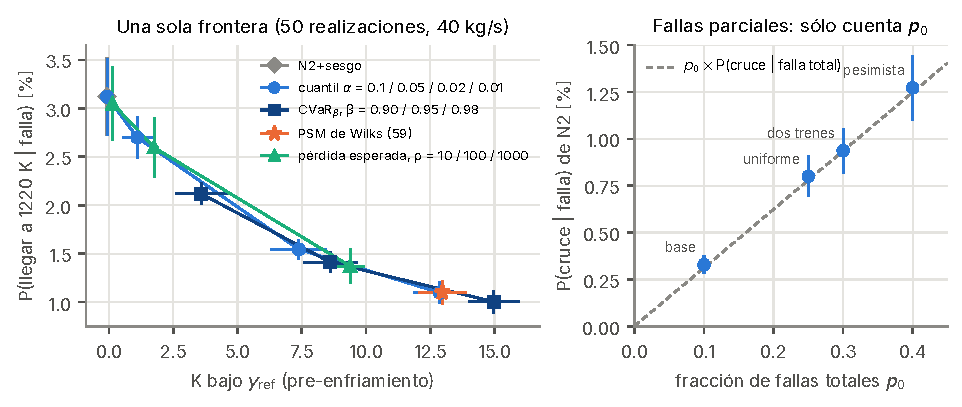
\includegraphics[width=\linewidth]{figures/fig_f6_frontier.pdf}
\caption{Izquierda: las cuatro familias de formulaciones sobre la misma curva
riesgo--pre-enfriamiento; barras: IC al 95~por ciento. Derecha: riesgo de N2 con fallas
parciales para cuatro vectores de severidad (sección~\ref{sec:riesgo-parciales}); cae sobre la
recta $p_0\times P(\text{cruce}\mid\text{falla total})$.}
\label{fig:f6-frontier}
\end{figure}

\paragraph{Cómo leer la tabla.}
\begin{enumerate}
  \item \textbf{Una sola frontera.} Para un mismo riesgo, todas piden el mismo pre-enfriamiento:
        Wilks 59 y el cuantil con $\alpha=0.01$ dan 0.0110 con 13.0 y 12.9~K; el CVaR$_{0.95}$, la
        pérdida esperada con $\rho=1000$ y el cuantil con $\alpha=0.02$ dan 0.014--0.016 con
        7.4--9.4~K. Ninguna es más eficiente; sólo cambia el parámetro con que se recorre la
        frontera ($\alpha$, $\beta$, $\rho$ o el tamaño de la muestra de Wilks).
  \item \textbf{Equivalencias.} El CVaR$_{0.95}$ equivale a un cuantil con $\alpha\approx0.015$, y
        Wilks 59 a uno con $\alpha\approx0.01$: el máximo de 59 sorteos es, en promedio, el
        cuantil $1-1/60\approx0.983$, con dispersión entre consultas.
  \item \textbf{Costo computacional.} Las cotas agregan una simulación del ROM y una restricción
        por paso ($\approx0.1$~s por consulta en el percentil 99). La pérdida esperada agrega
        $26\times40$ variables al QP ($\approx0.28$~s). Las cuatro siguen en tiempo real.
\end{enumerate}

\takeaway{\textbf{Respuesta a Q11.} La cota con cuantil. Es la más simple, su parámetro es una
probabilidad interpretable y su garantía se verificó. El CVaR conviene si el equipo prefiere
controlar la severidad de la cola en vez de su probabilidad, pero no compra más protección por
kelvin de pre-enfriamiento. Wilks agrega ruido entre consultas sin ganar eficiencia. El
resultado de Homem-de-Mello se cumple aquí en forma exacta: la decisión con riesgo es la de N2
determinista con un único escenario de falla $D^*$, el que hace que $\Delta T(D^*)$ sea el
margen.}

%======================================================================
\section{Fallas parciales}\label{sec:riesgo-parciales}
%======================================================================
\paragraph{Por qué podían cambiar la conclusión.} Con una falla total, la decisión no importa
durante la falla y todas las formulaciones se reducen a un margen. Con una falla parcial de
severidad $\eta$, la planta recibe $\eta\,u$: la incertidumbre \emph{multiplica} a la decisión.
Para una falla que empieza en el paso $j$ del horizonte,
$\hat y_k(u)=y_{0,k}+\sum_{i<j}G_{k,i}u_i+\eta\sum_{i\ge j}G_{k,i}u_i$, y el exceso ya no es
«predicción sin falla más una constante». Eso da formulaciones que no se reducen a una cota.

\paragraph{Modelo (supuesto; el DET no tiene fallas parciales).} Los instantes y las duraciones
salen de la familia del DET. Cada falla saca de 1 a 4 de 4 trenes paralelos:
$\eta\in\{0.75,0.5,0.25,0\}$, con probabilidades base $\{0.4,0.3,0.2,0.1\}$. Durante la falla, N2
empuja al máximo y la planta recibe $\eta\,\dot m_{\max}$. Se probaron tres formulaciones (en
\code{julia/f5b1d\_partial.jl}): la \textbf{cota con $\eta$}, $U=1220-m$ con
$\sum_\eta p_\eta P(\Delta T_\eta(D)>m)=\alpha$, y el \textbf{CVaR} y la \textbf{pérdida esperada con
escenarios dentro del horizonte} (inicio, $\eta$ y $D$), que no se reducen a una cota. El riesgo
se evalúa con Rao--Blackwell generalizado: $\sum_\eta p_\eta S(\tau_\eta(x_t))$, donde $\tau_\eta$ es
el tiempo del HRM hasta 1220~K con caudal $\eta\,\dot m_{\max}$.

\begin{figure}[H]\centering
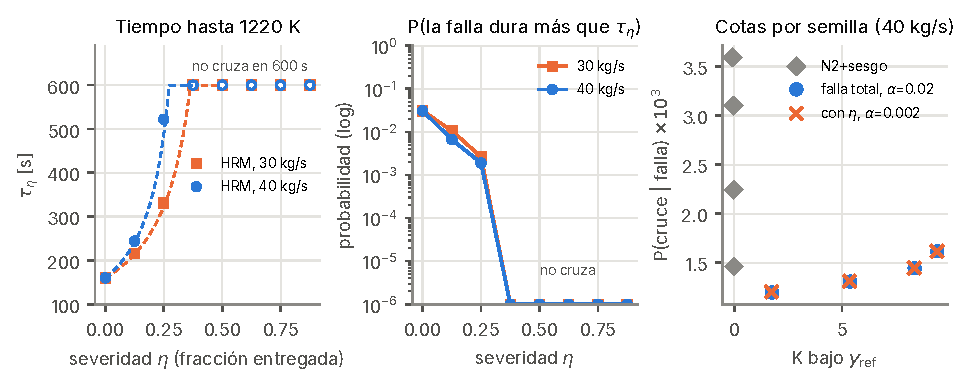
\includegraphics[width=\linewidth]{figures/fig_f5b_partial_failures.pdf}
\caption{Por qué las fallas parciales casi no agregan riesgo. Izquierda: tiempo hasta 1220~K en
el HRM si el ACS entrega $\eta\,\dot m_{\rm max}$ (puntos); la aproximación
$\tau_\eta\approx\tau_0/(1-\eta\,\dot m_{\rm max}/\mathrm{fuga})$ (trazos) lo reproduce con un error
menor que el 7~por ciento. Centro: probabilidad de que la falla dure más que $\tau_\eta$; con
$\eta\ge0.375$ la PCT no llega a 1220~K. Derecha: por semilla, la cota que conoce $\eta$ con
$\alpha=0.002$ coincide con la de falla total con $\alpha=0.02$.}
\end{figure}

\paragraph{Resultados} (50 realizaciones, campaña F6 \code{eta}; cuatro vectores de
probabilidades sobre $\eta=(0.75,0.5,0.25,0)$: base $(.4,.3,.2,.1)$, uniforme, pesimista
$(.1,.2,.3,.4)$ y dos trenes $(0,.7,0,.3)$).
\begin{enumerate}
  \item \textbf{El riesgo es $p_0$ veces el de las fallas totales.} El de N2 vale 0.0033
        (base, $p_0=0.1$), 0.0080 (uniforme, 0.25), 0.0094 (dos trenes, 0.3) y 0.0127
        (pesimista, 0.4): con tres cifras, $p_0\times0.031$ (figura~\ref{fig:f6-frontier},
        derecha). Las fallas parciales no aportan riesgo medible, que es el caso
        $\varepsilon\approx0$ de la proposición~\ref{prop:eta}.
  \item \textbf{Por qué.} Con caudal parcial, la PCT sube más lento y tarda más en llegar a
        1220~K. Como la duración es exponencial (media de 46~s), la probabilidad de que la falla
        dure más que ese tiempo cae exponencialmente con el retraso (figura anterior).
  \item \textbf{La cota con $\eta$} y $\alpha=0.01$ cumple su nivel con todos los vectores
        (0.0060 uniforme, 0.0065 dos trenes, 0.0072 pesimista; con el vector base queda
        inactiva, porque N2 ya está en 0.0033). Equivale a la cota de falla total con
        $\alpha/p_0$.
  \item \textbf{Las formulaciones con escenarios dentro del horizonte no actúan}: dan lo mismo
        que N2. El pico llega al final de la falla, casi siempre después de los 13~s del
        horizonte, así que la parte multiplicativa pesa poco.
\end{enumerate}

\takeaway{Con duraciones exponenciales, la cota de falla total sigue siendo la formulación
relevante. Basta fijar su $\alpha$ pensando en la fracción de fallas que son totales. La
estructura multiplicativa sólo importaría con duraciones de cola pesada, con fallas parciales
severas y frecuentes, o con una capacidad muy por debajo de la fuga.}

%======================================================================
\section{Sensibilidad y condición de aplicabilidad}\label{sec:riesgo-aplicabilidad}
%======================================================================
\paragraph{Qué supuestos se probaron.} Tres supuestos no los fijamos nosotros: la aceleración
de las reparaciones, la capacidad del ACS y las probabilidades de severidad (sección anterior).
La campaña F6 \code{sens} barrió los dos primeros en 50 realizaciones:
$\mu\times\{3\cdot10^3,10^4,3\cdot10^4\}$ por capacidad de 30, 35, 40, 45 y 50~kg/s. Como la
trayectoria de un controlador que no usa el modelo de fallas no depende de $\mu$, el riesgo de
Rao--Blackwell se evalúa para los tres $\mu$ en la misma corrida. Las cotas sí dependen de $\mu$
y se corrieron una vez por cada $\mu$ de diseño, lo que además mide qué pasa si $\mu$ está mal
especificado.

\begin{figure}[H]\centering
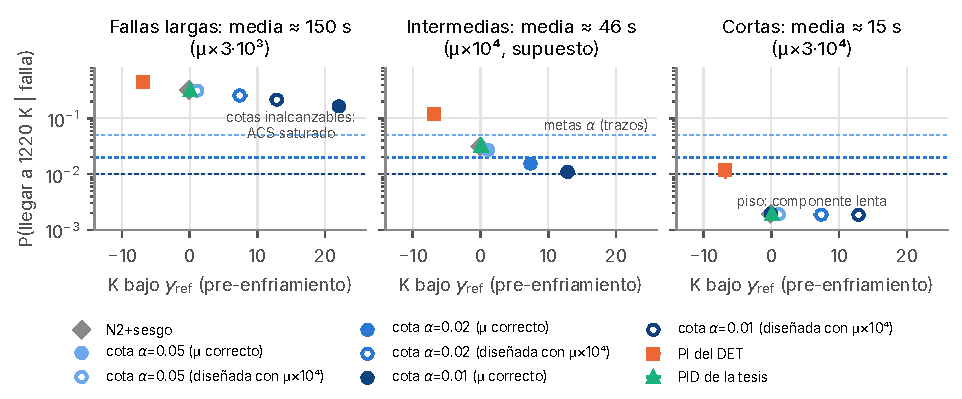
\includegraphics[width=\linewidth]{figures/fig_f6_regimes.pdf}
\caption{Riesgo frente a pre-enfriamiento a 40~kg/s, 50 realizaciones, para tres duraciones
medias de la falla. Puntos llenos: la cota diseñada con el $\mu$ verdadero. Puntos huecos: la cota
diseñada con $\mu\times10^4$ (error de especificación). Trazos: la meta $\alpha$ de cada cota.
Sólo en el panel central las cotas actúan y cumplen su meta.}
\end{figure}

\paragraph{Tres regímenes.} La duración media de la falla se compara con el tiempo que tarda la
PCT en llegar a 1220~K con el ACS apagado ($\tau\approx165$~s):
\begin{itemize}
  \item \textbf{Fallas largas} (media $\approx150$~s $\approx\tau$). Para cumplir $\alpha$ habría que
        bajar la PCT a $U_\alpha\approx920$--1070~K. Es imposible: el ACS se satura, pre-enfría
        22~K (+42\,\% de masa) y el riesgo baja de 0.32 a 0.16, todavía muy lejos de $\alpha$.
  \item \textbf{Fallas intermedias} (media $\approx46$~s, el caso base). Es el único régimen
        donde la cota actúa y cumple su meta (sección~\ref{sec:riesgo-rb}).
  \item \textbf{Fallas cortas} (media $\approx15$~s). $U_\alpha\ge1200$~K, por encima de la
        consigna, así que la cota nunca actúa. El riesgo es el piso de la componente lenta
        (0.0019).
\end{itemize}
El error de especificación no es simétrico. Una cota diseñada para fallas de 46~s que enfrenta
fallas más cortas sobra, pero no cuesta nada: queda inactiva. Si enfrenta fallas más largas, el
riesgo sube a 0.26 con $\alpha=0.02$ y pierde la garantía.

\paragraph{La capacidad del ACS casi no importa.} Entre 30 y 50~kg/s, N2 queda en 0.031 y la
cota con $\alpha=0.02$ en 0.0147--0.0174, con 6.6--7.7~K de pre-enfriamiento. Durante una falla
el caudal es cero sea cual sea la capacidad, así que es la duración la que fija el riesgo. La
única excepción es $\alpha=0.01$ a 30~kg/s (0.0138): con poca capacidad, la cota no se puede
cumplir en la fase aguda.

\paragraph{Qué significa físicamente la aceleración.} Una falla del ACS puede terminar por tres
mecanismos, con escalas de tiempo muy distintas:
\begin{center}\small
\begin{tabularx}{\linewidth}{@{}l Y l@{}}\toprule
Mecanismo & Escala de tiempo & Fuente\\\midrule
Reparación del componente & Días: las tasas reales del DET dan medias de 129~h, 70~h, 18~h y 3.4 años; en sistemas de metal líquido, una bomba tarda $\sim$33 días y una válvula 3 días & DET; \cite{cadwallader}\\
Recuperación por el operador & Decenas de minutos: los APS usan probabilidades de no recuperación de 0.25--0.3 a los 30--40~min & \cite{nrcgi122}\\
Recuperación automática por redundancia & Segundos a decenas de segundos: un equipo de reserva arranca y toma carga en 10~s, más el restablecimiento del caudal & \cite{nfpa110}\\\bottomrule
\end{tabularx}
\end{center}
Ninguna capa de control puede mitigar una falla que se termina por reparación o por acción del
operador: dura mucho más que $\tau$, y la PCT llega a 1220~K pase lo que pase. Esas fallas
pertenecen al análisis probabilístico de seguridad (frecuencia por consecuencia), no al MPC. El
MPC sólo puede proteger contra interrupciones que se \emph{recuperan automáticamente}. Por eso
el caso base $\mu\times10^4$ se interpreta como un \textbf{tiempo de recuperación automática}
$\bar t_{\rm rec}$: medias de 6.5--46~s, compatibles con un arranque de 10--20~s más el
restablecimiento del caudal. La componente de 2.9~h representa las fallas que no se recuperan
solas, el piso de riesgo. Falta el dato del equipo: si el ACS del SMDFR tiene trenes redundantes
con arranque automático, y cuánto tarda en restablecer el caudal.

\takeaway{\textbf{Respuesta a Q12.} La capa de riesgo sirve cuando el tiempo de recuperación
automática del ACS es comparable al tiempo que tarda la PCT en llegar a 1220~K sin enfriamiento,
pero menor: $\bar t_{\rm rec}\approx0.1$--$0.5\,\tau$. Si las fallas se recuperan mucho más
rápido, sobra; si duran tanto como $\tau$ o más, ningún controlador cumple $\alpha$ y el riesgo
pasa al APS. La capacidad del ACS y la severidad de las fallas parciales no cambian esta
conclusión.}

%======================================================================
\section{Lazo cerrado con fallas: las métricas de la tesis}\label{sec:riesgo-fallas}
%======================================================================
La última prueba aplica las fallas del DET dentro del lazo (no sólo en el estimador) y mide cada
controlador con las métricas de la tesis (sección~\ref{sec:desempeno}). Son 50 realizaciones a
40~kg/s, todas con al menos una falla (campaña F6 \code{det}).

\begin{table}[H]\centering\small\setlength{\tabcolsep}{3pt}
\begin{tabularx}{\linewidth}{@{}Y c r c r r r@{}}\toprule
Controlador & 1220~K & IAE [K\,s] & Se asienta & VT [kg/s] & DSM mín. & PCT pico\\\midrule
N1 = N2 = N3 (+sesgo) & 0/50 & $475\pm220$ & 60\,\% & 136 & 54.9~K & 1189~K\\
N2 + DSM de la tesis ($\lambda=10^4$) & 0/50 & 475 & 60\,\% & 138 & 54.9~K & 1189~K\\
N2 + pérdida esperada $\rho=100$ & 0/50 & $707\pm170$ & 0\,\% & 403 & 56.4~K & 1188~K\\
N2 + cota $\alpha=0.02$ & 0/50 & $1689\pm210$ & 0\,\% & 1483 & 59.3~K & 1185~K\\
N2 + CVaR$_{0.95}$ / Wilks 59 & 0/50 & 1926 / 2806 & 2 / 0\,\% & 1454 / 1711 & 59.7 / 60.6~K & 1184 / 1183~K\\
PID de la tesis & 1/50 & $1185\pm150$ & 2\,\% & 35\,650 & 52.1~K & 1192~K\\
PI del DET & 7/50 & $3293\pm170$ & 0\,\% & 63 & 34.8~K & 1209~K\\\bottomrule
\end{tabularx}
\caption{Métricas de la tesis en 50 realizaciones con fallas del DET (40~kg/s). «Se asienta»:
fracción que entra y queda en la banda de 0.30~K. VT: variación total del caudal mandado. DSM
mín.: margen mínimo a 1244~K.}
\label{tab:det-tesis}
\end{table}

\noindent La variación total de las capas de riesgo (1450--1710~kg/s) viene de una oscilación de
período dos del caudal. Una supresión de movimiento pequeña la elimina sin cambiar el riesgo,
el margen ni la masa (sección~\ref{sec:supresion}).

\noindent La tabla da promedios. La figura~\ref{fig:syn-fan} muestra las 50 trayectorias de cada
controlador alineadas en el inicio de la falla, que es donde se decide si se cruza o no 1220~K.

\begin{figure}[H]\centering
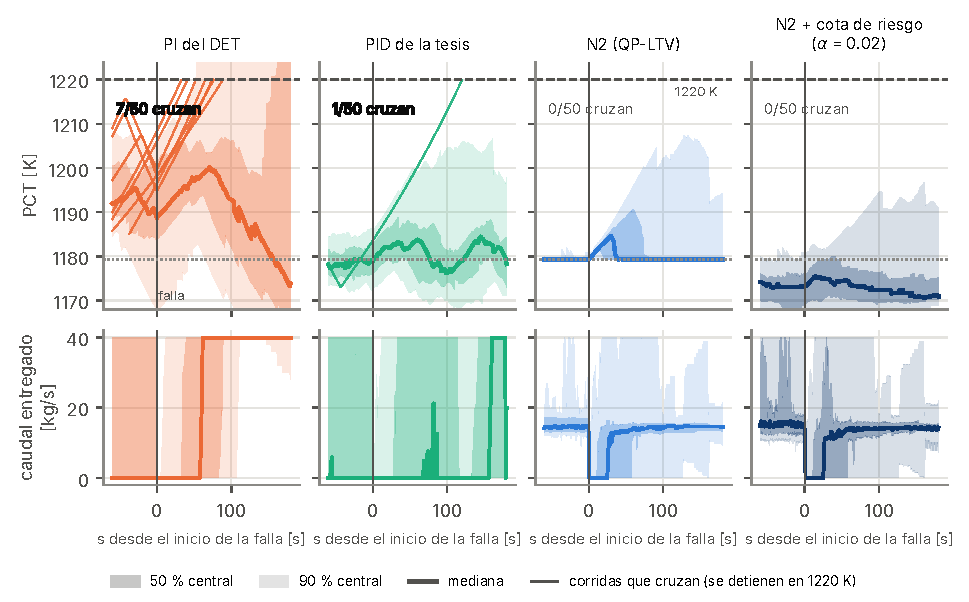
\includegraphics[width=\linewidth]{figures/syn_cl_fan.pdf}
\caption{Cincuenta lazos cerrados con fallas del DET (40~kg/s), alineados en el inicio de la
primera falla ($s=0$). Arriba, PCT; abajo, caudal que entrega el ACS (cero durante la falla).
Bandas: 50 y 90\,\% central por instante; línea gruesa: mediana. Las líneas finas son las corridas
que llegan a 1220~K, donde se detienen. En la mayoría de las realizaciones el PI del DET no
inyecta antes de la falla (zona muerta) y la PCT la recibe alta; la cota de riesgo trabaja
6--7~K bajo la consigna y ese margen absorbe las fallas largas.}
\label{fig:syn-fan}
\end{figure}

\paragraph{Cómo leer la tabla.}
\begin{enumerate}
  \item \textbf{Ninguna variante de N2 llega a 1220~K}; el PID de la tesis llega en una
        realización y el PI del DET en siete.
  \item \textbf{Las capas de riesgo suben el IAE a propósito.} Trabajan bajo la consigna para
        tener margen ante la próxima falla, y la métrica de la tesis cuenta ese margen como
        error de seguimiento. A cambio, el DSM mínimo sube de 54.9 a 59--61~K y la PCT pico baja
        4--6~K. Es el precio del margen, no un defecto de seguimiento.
  \item \textbf{El DSM de la tesis tampoco actúa con fallas}: la trayectoria es la misma que sin
        él, con un poco más de movimiento del actuador.
  \item \textbf{El PID de la tesis} tiene un IAE 2.5 veces el de N2, casi nunca se asienta y su
        caudal oscila (VT de 35\,650~kg/s). El PI del DET tiene un IAE 7 veces mayor y el menor
        margen.
\end{enumerate}

\takeaway{Con fallas reales en el lazo, N2, con o sin capa de riesgo, no cruza 1220~K en
ninguna realización, mientras que el PID y el PI de la tesis sí lo hacen. Las capas de riesgo cambian margen por
error de seguimiento en la cantidad que fija su parámetro, como predice la frontera.}
